\documentclass[10pt,xcolor=pdflatex]{beamer}
\usepackage{newcent}
\usepackage[utf8]{inputenc}
\usepackage[czech]{babel}
\usepackage{hyperref}
\usepackage{textpos}
\usepackage{multicol}
\usepackage{tikz}
\usepackage{fancyvrb}
\usepackage{color}
\usepackage{subfig}
\usepackage{geometry}
\usepackage{graphicx}
\usepackage{epstopdf}


\usepackage{todonotes}
\usepackage{listings}

\makeatletter
\g@addto@macro{\UrlBreaks}{\UrlOrds}
\makeatother

\newcommand{\emp}{\lstinline[language={[LaTeX]TeX}, basicstyle=\tt\color{fitdark}]}

\lstdefinelanguage{XML}
{
  basicstyle=\ttfamily\footnotesize,
  morestring=[b]",
  moredelim=[s][\color{red!70!black}]{<}{\ },
  moredelim=[s][\color{red!70!black}]{</}{>},
  moredelim=[l][\color{red!70!black}]{/>},
  moredelim=[l][\color{red!70!black}]{>},
  morecomment=[s]{<?}{?>},
  morecomment=[s]{<!--}{-->},
  commentstyle=\color{black},
  stringstyle=\color{brown!80!black},
  identifierstyle=\color{violet}
}
\lstset{language=Java,
  showspaces=false,
  showtabs=false,
  breaklines=true,
  showstringspaces=false,
  breakatwhitespace=true,
  commentstyle=\color{green!70!black},
  keywordstyle=\color{blue},
  stringstyle=\color{red},
  basicstyle=\ttfamily,
  moredelim=[il][\textcolor{darkgrey}]{\$\$},
  moredelim=[is][\textcolor{darkgrey}]{\%\%}{\%\%}
}

\newcommand{\inlinejava}{\lstinline[language={Java},basicstyle=\ttfamily,keepspaces]}
\newcommand{\inlinejavaEmp}{\color{fitdark}\lstinline[language={Java},basicstyle=\ttfamily,keepspaces]}
\newcommand{\inlinexml}{\lstinline[language={XML},basicstyle=\ttfamily,keepspaces]}
\newcommand{\itmspace}[2]{\item #2 \vspace{#1}}
\newcommand{\tabright}[2]{\dotfill\begin{tabular}[t]{l}{#1}\hspace*{#2}\end{tabular}}
\newcommand{\bcirc}{\tikz\draw[fitblue, fill=fitblue] (0,0) circle (.35ex);}

\newcommand{\radkovani}[1]{\renewcommand{\baselinestretch}{#1}}
\newcommand{\file}[1]{\texttt{#1}}

\epstopdfDeclareGraphicsRule{.gif}{png}{.png}{convert gif:#1 png:\OutputFile}
\AppendGraphicsExtensions{.gif}
\usetheme{FIT}

\def\uv#1{\quotedblbase#1\textquotedblleft}%
\newcommand{\putat}[3]{\begin{picture}(0,0)(0,0)\put(#1,#2){#3}\end{picture}}

%%%%%%%%%%%%%%%%%%%%%%%%%%%%%%%%%%%%%%%%%%%%%%%%%%%%%%%%%%%%%%%%%%
\title[GJA 10]{Android advanced}

\author[]{Jaroslav Dytrych}

\institute[]{Faculty of Information Technology
Brno University of Technology \\
Bo\v{z}et\v{e}chova 1/2. 612 66 Brno - Kr\'alovo Pole\\
dytrych@fit.vut.cz}

\date{4 December 2023}
%\date{\today}
%\date{} % bez data

%%%%%%%%%%%%%%%%%%%%%%%%%%%%%%%%%%%%%%%%%%%%%%%%%%%%%%%%%%%%%%%%%%

\begin{document}

\frame[plain]{\titlepage}

\begin{frame}[fragile]\frametitle{Content}
\begin{itemize}
	\item Interacting with other Apps
	\item Content sharing
	\item Background jobs
	\item Google Maps and Location API
	\item Google Play Services
	\item Location API
	\item Maps API
\end{itemize}
\end{frame}


\begin{frame}[fragile]\frametitle{Interaction}
\begin{itemize}
	\item Explicit intents are only for remote services.
	\item Otherwise implicit intents must be used.
	\item Simple intents
      \begin{itemize}
    	\item Make a call.
		\item View a webpage or a map.
		\item \ldots
      \end{itemize}
    \item Intents with extras
      \begin{itemize}
    	\item Compose an email.
		\item Create calendar event.
        \item \ldots
      \end{itemize}
\end{itemize}
\end{frame}


\begin{frame}[fragile]\frametitle{Interaction}
\begin{itemize}
	\item Verify your intent can be handled
	  \lstset{language=Java, basicstyle=\footnotesize\ttfamily}
            \begin{lstlisting}
PackageManager packageManager = getPackageManager();
List<ResolveInfo> activities = 
packageManager.queryIntentActivities(intent, 0);
boolean isIntentSafe = activities.size() > 0;
            \end{lstlisting}
    \item Default chooser appears, when multiple apps can handle your intent.
	\item Handle result of an App
      \begin{itemize}
    	\item \texttt{startActivityForResult(intent)}
		\item Override \texttt{OnActivityResult()} callback.
		\item Resolve which result it is by \texttt{REQUEST\_ID}.
		\item Query content resolver.
      \end{itemize}
\end{itemize}
\end{frame}


\begin{frame}[fragile]\frametitle{Interaction}
\begin{itemize}
	\item Allow other apps to start your activity.
	  \begin{itemize}
		\item Utilize intent filter.
          \begin{itemize}
            \item Action
            \item Data (mime type)
	        \item Category
          \end{itemize}
	  \end{itemize}
      \begin{itemize}
    	\item Handle request in \texttt{onCreate} method.
		\item Return back results with \texttt{setResult} function.
		\item Call \texttt{finish()} on your activity.
      \end{itemize}
\end{itemize}
\begin{textblock}{15}(6.5,4.5)
    {\footnotesize Example AndroidInteraction, CalledActivity}
\end{textblock}
\end{frame}


\begin{frame}[fragile]\frametitle{Content sharing}
\begin{itemize}
	\item Data can be sent to other Apps via extras
	  \begin{itemize}
		\item \texttt{EXTRA\_TEXT}
		\item \texttt{EXTRA\_STREAM} -- URI (e.g. to image data)
	  \end{itemize}
    \item Receiving data
	  \begin{itemize}
		\item Intent filters  \texttt{ACTION\_SEND}(\texttt{\_MULTIPLE})
		\item Mime type must be defined.
	  \end{itemize}
    \item File sharing
	  \begin{itemize}
		\item Declare file provider in manifest.
		\item Specify sharing paths.
		\item Accessible via
        \item[] \begin{footnotesize}\verb;content://name.of.package.fileprovider/sharingpath/; \end{footnotesize}
        \item[] \begin{footnotesize}\verb;default_image.jpg; \end{footnotesize}
	  \end{itemize}
\end{itemize}
\end{frame}


\begin{frame}[fragile]\frametitle{Content sharing}
\begin{itemize}
	\item File provider must specify intent filter.
	  \begin{itemize}
		\item \texttt{ACTION\_PICK}
		\item Category \texttt{OPENABLE}
      \end{itemize}
    \item Requesting App gets data via URI.
	\item Usually more Apps can supply files.
      \begin{itemize}
        \item Explicit App can be called directly.
	    \item Avoid chooser by Intent's 
        \item[] \texttt{setComponentName(package, full class name)}
      \end{itemize}
\end{itemize}
\begin{textblock}{15}(8.1,4.2)
    {\footnotesize Examples FileProvider, FileRequest}
\end{textblock}
\end{frame}


\begin{frame}[fragile]\frametitle{Android drawing}
\begin{itemize}
  \item Simple
    \begin{itemize}
      \item Class must extend \texttt{View}
      \item \texttt{onDraw()} -- repaints whole view
      \item \texttt{invalidate()}
    \end{itemize}
  \item SurfaceView
    \begin{itemize}
      \item \texttt{onDraw()} -- called manually, draws on holder's canvas.
      \item Drawing performed via thread.
    \end{itemize}
  \item Advanced graphics
    \begin{itemize}
      \item OpenGL ES
      \item \texttt{GLSurfaceView}
    \end{itemize}
\end{itemize}
\begin{textblock}{15}(7.6,3.4)
    {\footnotesize Examples StartDraw, HelloOpenGLES}
\end{textblock}
\end{frame}


\begin{frame}[fragile]\frametitle{Background Jobs}
\begin{itemize}
	\item Several possibilities in Android
	  \begin{itemize}
		\item Services
          \begin{itemize}
            \item Local
	        \item External
          \end{itemize}
    	\item \texttt{ThreadPoolExecutor}
          \begin{itemize}
            \item Queue of Runnables.
	        \item Method \texttt{poll()} for obtaining \texttt{Runnable} resource.
	        \item \texttt{execute(Runnable)} to start the task in background.
          \end{itemize}
        \item \texttt{AsyncTask}
      \end{itemize}
\end{itemize}
\end{frame}


\begin{frame}[fragile]\frametitle{Background Jobs}
\begin{itemize}
	\item \verb;AsyncTask<Params,Progress,Result>;
	\item \texttt{Params} -- List of “settings” objects, telling AsyncTask what to do.
	\item \texttt{Progress} -- can be returned via \texttt{publishProgress(Progress)}
	\item \texttt{Result} -- return type of result.
    \item 4 steps of processing.
\end{itemize}
\end{frame}


\begin{frame}[fragile]\frametitle{Background Jobs}
\begin{itemize}
	\item \texttt{AsyncTask} -- continuation
	  \begin{itemize}
		\item \texttt{OnPreExecute}
          \begin{itemize}
            \item invoked on the UI thread
            \item initialization
          \end{itemize}
    	\item \texttt{Result doInBackground(Progress \ldots)}
          \begin{itemize}
            \item after \texttt{onPreExecute} finishes processing
          \end{itemize}
    	\item \texttt{void onProgressUpdate(Progress)}
          \begin{itemize}
            \item invoked by \texttt{publishResults()}
	        \item on UI thread -- can update views
          \end{itemize}
      \end{itemize}
	\item Can be cancelled
      \begin{itemize}
    	\item Method \texttt{cancel(boolean mayInterruptIfRunning)}
        \item \texttt{OnCancelled} called instead of \texttt{onPostExecute}
      \end{itemize}
\end{itemize}
\end{frame}

\begin{frame}[fragile]\frametitle{Background Jobs}
\begin{itemize}
	\item \texttt{AsyncTask} is deprecated in favour of  standard \texttt{java.util.concurrent} or Kotlin concurrency utilities (Kotlin coroutines).
\end{itemize}
{\footnotesize 
\begin{lstlisting}
    ExecutorService executor = Executors.newSingleThreadExecutor();
    Handler handler = new Handler(Looper.getMainLooper());

    executor.execute(() -> {
        // Background work here
        handler.post(() -> {
            // UI Thread work here
        });
    });
\end{lstlisting}
}
\end{frame}




\begin{frame}[fragile]\frametitle{Google Maps and Location API}
\begin{itemize}
	\item Must use Google Play Services.
   	\item Can be referenced as LibraryProject\newline \begin{footnotesize}
   	\verb;<meta-data android:name="com.google.android.gms.version";\newline
\verb;android:value="@integer/google_play_services_version" />;\end{footnotesize}	
	\item Usually present on nowadays android devices, but programmer should check.
	\item Needs extra libraries for emulator.
	  \begin{itemize}
		\item \texttt{com.android.vending.apk}
		\item \texttt{com.google.android.gms.apk}
	  \end{itemize}
    \item Some emulators have them preinstalled (marked with icon).
\end{itemize}
\end{frame}


\begin{frame}[fragile]\frametitle{Google Play Services}
\begin{itemize}
	\item Google Play Services runs on device with Android 2.3 and higher.
	  \begin{itemize}
		\item Emulator 4.2.2 and higher \newline\begin{footnotesize} \verb|GooglePlayServicesUtil.isGooglePlayServicesAvailable(this);|\end{footnotesize}\newline
		on newer versions:
		\newline\begin{footnotesize} \verb|GoogleApiAvailability.isGooglePlayServicesAvailable(this);|\end{footnotesize}
        \item Interfaces must be implemented \newline \begin{footnotesize}
\verb;GooglePlayServicesClient.ConnectionCallbacks,;
\verb;GooglePlayServicesClient.OnConnectionFailedListener;
\end{footnotesize}\newline
on newer versions:\newline \begin{footnotesize}
\verb;GoogleApiClient.ConnectionCallbacks,;
\verb;GoogleApiClient.OnConnectionFailedListener;
\end{footnotesize}
		\item Respective callbacks
		  \begin{itemize}
		    \item \texttt{OnConnected}
	        \item \texttt{OnConnectionFailed}
	        \item \texttt{OnDisconnected}
	        \item \texttt{onConnectionSuspended}
		  \end{itemize}
	  \end{itemize}
\end{itemize}
\end{frame}


\begin{frame}[fragile]\frametitle{GooglePlayServices}
\putat{-28}{-103}{
    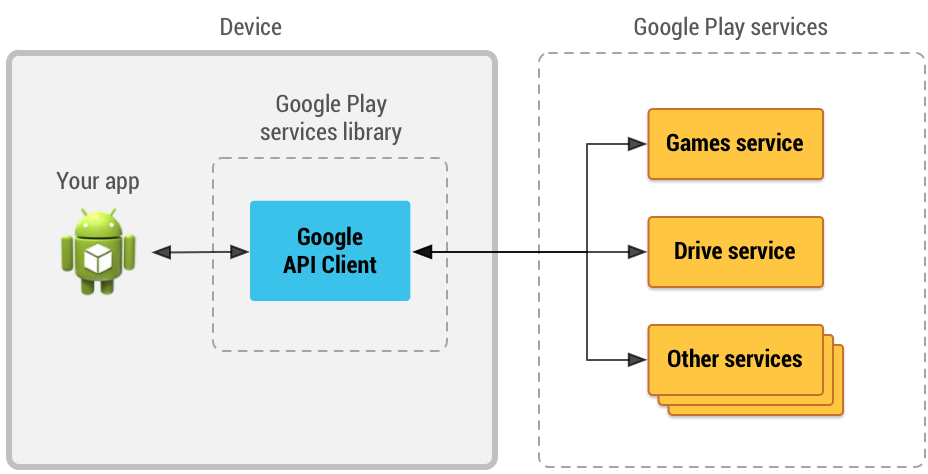
\includegraphics[scale=0.382]{img/pic5.png}
}
\begin{textblock}{15}(5.1,6.5)
    {\footnotesize Asynchronous communication}
\end{textblock}
\end{frame}


\begin{frame}[fragile]\frametitle{GooglePlayServicesClient deprecated}
\begin{itemize}
  \item Rather than tacking multiple APIs onto a single API client, each API now has a purpose-built client object class that extends \texttt{GoogleApi}. Unlike with \texttt{GoogleApiClient} there is no performance cost to creating many client objects. Each of these client objects abstracts the connection logic, connections are automatically managed by the SDK in a~way that maximizes both speed and efficiency.
  \begin{itemize}
      \item e.g. \texttt{DriveResourceClient}
  \end{itemize}
\end{itemize}
\end{frame}


\begin{frame}[fragile]\frametitle{Google Play Services}
\putat{-23}{-130}{
    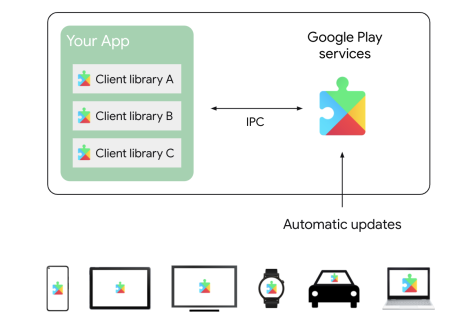
\includegraphics[scale=0.9]{img/play-services-diagram.png}
}
\begin{textblock}{15}(-0.6,7.3)
    {\footnotesize Google Play services receives regular updates that contain improvements and bug fixes.}
\end{textblock}
\end{frame}


\begin{frame}[fragile]\frametitle{Location API}
\begin{itemize}
	\item Location API must declare permission
	  \begin{itemize}
		\item \texttt{ACCESS\_COARSE\_LOCATION}
		\item \texttt{ACCESS\_FINE\_LOCATION}
	  \end{itemize}
	\item \texttt{LocationServices.FusedLocationProviderApi} \newline or
	      \texttt{FusedLocationProviderClient}
      \begin{itemize}
        \item entry point for interacting with the fused location provider.
      \end{itemize}
	\item Current location can be obtained via client using method
    \item[] \begin{footnotesize}
      \makebox[\linewidth][l]{\texttt{getLastLocation();}}
      \end{footnotesize}
    \item Application can handle location updates.
\end{itemize}
\end{frame}


\begin{frame}[fragile]\frametitle{Location API}
\begin{itemize}
	\item Location updates
	  \begin{itemize}
		\item Programmer must form \texttt{LocationRequest} object.
	  \end{itemize}
    \item Accuracy
	\item Update interval \newline \begin{footnotesize}\verb|locationClient.requestLocationUpdates(locationRequest, Context);|\end{footnotesize}
    \item Location update callback
    \item[] 
	\lstset{language=XML, basicstyle=\footnotesize\ttfamily}
    \begin{lstlisting}
 @Override
  public void onLocationChanged(Location location) {
    // Report to the UI that the location was updated
    String msg = "Updated Location: " +
        Double.toString(location.getLatitude()) + "," +
        Double.toString(location.getLongitude());
    Toast.makeText(this, msg, Toast.LENGTH_SHORT).show();
  }
    \end{lstlisting}    
\end{itemize}
\end{frame}


\begin{frame}[fragile]\frametitle{Location API}
\begin{itemize}
	\item Can be used to convert location to address.
	\item Address computation can take some time.
	  \begin{itemize}
		\item It can't be done in UI thread.
	  \end{itemize}
    \item Addresses can be obtained from Geocoder object.
	  \begin{itemize}
		\item Address object can be used to get
          \begin{itemize}
            \item State
	        \item Administrative unit
	        \item Locality (usually city)
	        \item Sub-locality
	        \item Street
	        \item Address line
	        \item Phone (if known)
	        \item Postal code
          \end{itemize}
	  \end{itemize}
\end{itemize}
\begin{textblock}{15}(9.4,2.7)
    {\footnotesize Example AndroidLocation}
\end{textblock}
\end{frame}

\begin{frame}[fragile]\frametitle{Location API}
\begin{itemize}
	\item Geofences
	  \begin{itemize}
        \item points of interest.
		\item user location combined with nearby features.
		\item Geofence is rather an area.
	  \end{itemize}
    \item Geofence consists of
	  \begin{itemize}
		\item longitude, latitude, radius,
		\item expiration time, Geofence ID, Transition Type.
	  \end{itemize}
    \item Geofence storage
      \begin{itemize}
    	\item holds defined geofences.
      \end{itemize}
    \item Intent can be defined to handle transitions
      \begin{itemize}
    	\item \texttt{OnAddGeofencesResultListener}
		\item \texttt{OnHandleIntent} -- programmer can make updates in the App based on transition type.
      \end{itemize}
    \item Geofence monitoring can be turned off.
\end{itemize}
\end{frame}

\begin{frame}[fragile]\frametitle{Location API}
\begin{itemize}
	\item Recognizing user current activity
	  \begin{itemize}
		\item On foot
		\item Tilting
		\item In vehicle
		\item Riding a bike
		\item Running
		\item Walking
	  \end{itemize}
    \item Permission \texttt{ACTIVITY\_RECOGNITION}
      \begin{itemize}
    	\item Requires \texttt{ACCESS\_FINE\_LOCATION}
      \end{itemize}
    \item Registered \texttt{ActivityRecognitionClient} makes programmer-defined \texttt{IntentService} receive updates.
	\item Detected activity has method \texttt{describeContents}
      \begin{itemize}
    	\item can return confidence.
      \end{itemize}
\end{itemize}
\end{frame}


\begin{frame}[fragile]\frametitle{Maps API}
\begin{itemize}
	\item Programmer must get API key.
      \begin{itemize}
    	\item Accessible in Google API console
    	\item[] \url{https://console.cloud.google.com/apis/}
		\item Registered App must enable Maps API.
          \begin{itemize}
            \item Key can be generated for WebApp, Android, iOS device and server. 
               \lstset{language=XML, basicstyle=\footnotesize\ttfamily}
                    \begin{lstlisting}
<meta-data android:name="com.google.android.maps.v2.API_KEY"
    android:value="your api key"/>
\end{lstlisting}    
          \end{itemize}
      \end{itemize}
    \item Defined in manifest
      \begin{itemize}
   	 	\item Key can be generated in combination with SHA1 hash from local keystore (can be created within IDE when exporting apk).
      \end{itemize}
\end{itemize}
\end{frame}


\begin{frame}[fragile]\frametitle{Maps API}
\begin{itemize}
	\item Debug key
	  \begin{itemize}
		\item Key must be named “androiddebugkey”.
		\item Password both to keystore and key must be “android”.
	  \end{itemize}
    \item Release key
      \begin{itemize}
    	\item Private key must be generated
         \lstset{language=XML, basicstyle=\footnotesize\ttfamily}
          \begin{lstlisting}
keytool -genkey -v -keystore my-release-key.keystore
-alias alias_name -keyalg RSA -keysize 2048 
-validity 10000
          \end{lstlisting}   
    	\item Then can be application compiled.
        \item At the end -- APK must be signed with the key
         \lstset{language=XML, basicstyle=\footnotesize\ttfamily}
          \begin{lstlisting}
jarsigner -verbose -sigalg SHA1withRSA -digestalg SHA1
-keystore my-release-key.keystore my_application.apk alias_name
\end{lstlisting}   
      \end{itemize}
\end{itemize}
\end{frame}


\begin{frame}[fragile]\frametitle{Maps API}
\begin{itemize}
  \item Using predefined map fragments
\lstset{language=XML, basicstyle=\footnotesize\ttfamily}
\begin{lstlisting}
<?xml version="1.0" encoding="utf-8"?>
<FrameLayout xmlns:android="http://schemas.android.com/apk/res/android"
    android:layout_width="match_parent"
    android:layout_height="match_parent">
  <fragment
    android:id="@+id/map"
    android:layout_width="match_parent"
    android:layout_height="match_parent"
    android:tag="maps"    
    android:name="com.google.android.gms.maps.SupportMapFragment"
    />
</FrameLayout>
\end{lstlisting}  
  \item \texttt{MapFragment} supported in API \textgreater =12
    \begin{itemize}
	  \item \texttt{SupportMapFragment} for older versions.
    \end{itemize}
  \item \texttt{MapView} -- for embedding as View.
\end{itemize}
\end{frame}


\begin{frame}[fragile]\frametitle{Maps API}
\begin{itemize}
	\item Map types
	  \begin{itemize}
		\item Normal -- typical road map, important natural features such as rivers are shown.
		\item Hybrid -- satellite photograph data with road maps.
		\item Satellite -- raw satellite photograph data.
		\item Terrain -- topographic data. The map includes colors, contour lines and labels, and perspective shading.
		\item None -- the map will be rendered as an empty grid with no tiles loaded.
	  \end{itemize}
    \item Indoor maps -- floor plans can be added to Google maps directly, it will be visible for all users.
\end{itemize}
\begin{textblock}{15}(10.0,3.1)
    {\footnotesize Example AndroidMaps}
\end{textblock}
\end{frame}

\begin{frame}[fragile]\frametitle{Maps API}
  \begin{itemize}
	\item Map fragments can be added dynamically
	  \lstset{language=Java, basicstyle=\footnotesize\ttfamily}
      \begin{lstlisting}
mMapFragment = MapFragment.newInstance();
FragmentTransaction fragmentTransaction =
    getFragmentManager().beginTransaction();
fragmentTransaction.add(R.id.my_container, mMapFragment);
fragmentTransaction.commit();
\end{lstlisting} 
    \item Check map availability
      \lstset{language=Java, basicstyle=\footnotesize\ttfamily}
      \begin{lstlisting}
mMap = ((MapFragment) getFragmentManager().findFragmentById(R.id.map))
        .getMap();
    // Check if we were successful in obtaining the map.
    if (mMap != null) {
        // The Map is verified. It is now safe to 
        // manipulate the map.

    }
\end{lstlisting} 
\end{itemize}
\end{frame}


\begin{frame}[fragile]\frametitle{Maps API}
\begin{itemize}
	\item Map state
	  \begin{itemize}
		\item Camera position
          \begin{itemize}
            \item Location
	        \item Zoom
	        \item Bearing
	        \item Tilt
          \end{itemize}
    	\item Map type
		\item Controls and gestures
      \end{itemize}
    \item Can be defined in xml layout file or programatically.
\end{itemize}
\end{frame}


\begin{frame}[fragile]\frametitle{Maps API}
\begin{itemize}
	\item State configuration on XML layout file
      \lstset{language=Java, basicstyle=\footnotesize\ttfamily}
      \begin{lstlisting}
xmlns:map="http://schemas.android.com/apk/res-auto"
\end{lstlisting}
    \item Configuration via map namespace
      \lstset{language=Java, basicstyle=\footnotesize\ttfamily}
      \begin{lstlisting}
map:cameraBearing="112.5"
map:cameraTargetLat="-33.796923"
map:cameraTargetLng="150.922433"
map:cameraTilt="30"
map:cameraZoom="13"
map:mapType="normal"
\end{lstlisting}
    \item Programatic configuration
      \lstset{language=Java, basicstyle=\footnotesize\ttfamily}
      \begin{lstlisting}
GoogleMapOptions options = new GoogleMapOptions();
options.mapType(GoogleMap.MAP_TYPE_SATELLITE)
    .compassEnabled(false)
    .rotateGesturesEnabled(false)
    .tiltGesturesEnabled(false);
\end{lstlisting}
\end{itemize}
\end{frame}


\begin{frame}[fragile]\frametitle{Maps API}
\begin{itemize}
	\item Drawing on the map
      \begin{itemize}
    	\item Markers
		  \lstset{language=Java, basicstyle=\footnotesize\ttfamily}
          \begin{lstlisting}
mMap = ((MapFragment) 
  getFragmentManager().findFragmentById(R.id.map)).getMap();
mMap.addMarker(new MarkerOptions()
    .position(new LatLng(10, 10))
    .title("Hello world"));
\end{lstlisting}
      \end{itemize}
    \item Properties like \texttt{title}, \texttt{position}, \texttt{alpha}, \texttt{draggable}, \texttt{icon}, \texttt{snippet}, \texttt{visible}, \texttt{location}, \texttt{flag}, \texttt{color}, \texttt{image}, \texttt{rotation}.
    \item Markers can be animated
      \begin{itemize}
    	\item Info windows
          \begin{itemize}
            \item Only one displayed at the time.
	        \item Method of a marker.
          \end{itemize}
    	\item Overlays
          \begin{itemize}
            \item Ground -- drawing image on the map.
	        \item Tile -- grid with coordinates and zoom level.
          \end{itemize}
      \end{itemize}
\end{itemize}
\end{frame}


\begin{frame}[fragile]\frametitle{Maps API}
\begin{itemize}
	\item Drawing shapes
	  \begin{itemize}
		\item Polyline
		\item Polygon
          \begin{itemize}
            \item Shapes are autocompleted.
          \end{itemize}
    	\item Circles
		\item Z-index may be specified.
      \end{itemize}
    \item StreetView
\lstset{language=Java, basicstyle=\footnotesize\ttfamily}
\begin{lstlisting}
<fragment
 android:id="@+id/streetviewpanorama"
 android:layout_width="match_parent"
 android:layout_height="match_parent"
 class="com.google.android.gms.maps.StreetViewPanoramaFragment"/>
\end{lstlisting}
\item Enable/disable user navigation.
\end{itemize}
\end{frame}

\begin{frame}[fragile]\frametitle{Maps API}
\begin{itemize}
	\item Interacting with a map
	  \begin{itemize}
		\item UI controls
        \begin{itemize}
          \item Zoom controls
          \item Compass
	      \item My Location button
	      \item Level picker
        \end{itemize}
    	\item Map gestures
          \begin{itemize}
            \item Zoom
	        \item Scroll
	        \item Tilt
	        \item Rotate
          \end{itemize}
    	\item Events
          \begin{itemize}
            \item Click/Long Click
	        \item Camera change 
          \end{itemize}
      \end{itemize}
\end{itemize}
\end{frame}

\begin{frame}[fragile]\frametitle{References 1/2}
\begin{itemize}
	\item \url{https://developer.android.com/training/index.html}
	\item \url{https://developers.google.com/android/guides/overview}
	\item \url{https://developers.google.com/android/reference/packages}
	\item \url{https://developers.google.com/maps/gmp-get-started}
	\item \url{https://developers.google.com/maps/documentation/geolocation/overview}
	\item \url{https://cloud.google.com/maps-platform/}
	\item \url{https://stackoverflow.com/questions/58767733/android-asynctask-api-deprecating-in-android-11-what-are-the-alternatives}
	\item \url{https://android-developers.googleblog.com/2017/11/moving-past-googleapiclient_21.html}
        \item \url{https://stackoverflow.com/questions/13702117/how-can-i-handle-map-move-end-using-google-maps-for-android-v2}
\end{itemize}
\end{frame}

\begin{frame}[fragile]\frametitle{References 2/2}
\begin{itemize}
        \item \url{https://stackoverflow.com/questions/58381078/error-for-android-emulator-deciding-if-gldirectmem-vulkan-should-be-enabled}
\end{itemize}
\end{frame}

\bluepage{Thank you for your attention!}



\end{document}
